\documentclass[12pt,a4paper]{article}

% ── Packages ──
\usepackage[utf8]{inputenc}
\usepackage[T1]{fontenc}
\usepackage{amsmath,amssymb,amsfonts}
\usepackage{graphicx}
\usepackage{booktabs}
\usepackage{algorithm}
\usepackage{algpseudocode}
\usepackage[margin=2.5cm]{geometry}
\usepackage{hyperref}
\usepackage{cite}
\usepackage{xcolor}
\usepackage{caption}
\usepackage{subcaption}
\usepackage{multirow}
\usepackage{float}

\hypersetup{colorlinks=true, linkcolor=blue, citecolor=blue, urlcolor=blue}

\title{\textbf{Reinforcement Learning Based Adaptive Data Rate Optimization \\for LoRaWAN Networks Under Dense Deployment Scenarios}}
\author{Team Ping Floyd}
\date{\today}

\begin{document}
\maketitle

\begin{abstract}
This document present an approach to optimize the Adaptive Data Rate (ADR) mechanism in LoRaWAN networks using reinforcement learning (RL) methods. In dense IoT deployment where many devices transmit frequently in close radius, packet losses happen due to collisions and interference. The classical ADR algorithm that LoRaWAN use cannot adapt well to these dynamic conditions. We model the problem as a Markov Decision Process and apply three RL algorithms (Double Deep Q-Network with Prioritized Experience Replay (DDQN-PER), Proximal Policy Optimization (PPO), and Multi-Agent Reinforcement Learning (MARL)) to dynamically adjust spreading factor (SF) and transmission power (TP) for each device. We build the simulation environment on top of ns-3 network simulator with realistic interference from WiFi and LTE mobile devices. Our results show that RL based ADR can achieve up to 99.65\% packet delivery rate compare to 40\% with classical ADR in dense scenarios, while MARL provide significant energy savings. We also implement a physical testbed using ESP32 devices with SX1278 LoRa modules and a STM32 based gateway to validate our approach in real world.
\end{abstract}

\tableofcontents
\newpage

% ============================================================================
\section{Introduction}
\label{sec:introduction}
% ============================================================================

With the fast development of artificial intelligence in the recent years, using AI-based solutions in network environments is becoming more and more practical. It is no longer a question of whether AI will be used in networking, but rather where exactly it can be applied properly. The key thing is to identify the problems that naturally fit the structure of what AI algorithms need. specifically, problems that can be formulated as sequential decision making tasks.

One such natural fit is the Markov Decision Process (MDP). In an MDP, an agent observe the current state of the environment, take an action, receive a reward, and move to a next state. The goal is to learn a policy that maximize the cumulative reward over time. Now the important question is: where do we find such Markov Decision Problems in real networking scenarios?

If we take LoRaWAN, which is one of the most popular Low Power Wide Area Network (LPWAN) technologies for Internet of Things (IoT) applications, there is a very clear problem. LoRaWAN networks suffer from significant packet losses in dense deployment. This happen because of several reasons:

\begin{itemize}
    \item \textbf{Self-interference}: Multiple LoRa devices that use the same spreading factor on the same channel at the same time cause collisions. When two packets overlap in time and frequency, both are typically lost.
    \item \textbf{Congestion}: As the number of devices grow, the probability of collision increase exponentially. In the ALOHA like access scheme that LoRaWAN use, this is a fundamental problem.
    \item \textbf{External interference}: WiFi networks, LTE devices, and other radio sources in the ISM band create additional noise that reduce the signal to noise ratio (SNR).
\end{itemize}

This problem become especially severe when many devices are deployed within a radius of 0 to 1 kilometer from the gateway. In such dense deployments, the devices are all competing for the same limited radio resources, and the interaction between their transmission parameter choices create a dynamic environment that change constantly.

With Industry 4.0 and the increasing trend of smart factories, smart cities, and environmental monitoring, there is a growing need to deploy many sensors that send data frequently. When we have 20 or 30 devices transmitting every 10 to 60 seconds, the network become a competitive game where each device's action affect the performance of others. This is exactly where we can identify the Markov game structure.

Now, let us consider the alternative approach. Suppose we find a way to predict packet loss using traditional machine learning methods. recurrent neural networks, random forests, or other supervised learning techniques. We can predict with high accuracy that a packet is going to be lost. But then what? We know the loss will happen, but we do not have a mechanism to prevent it. Prediction alone is not enough. What we need is a system that can take action. change the spreading factor, adjust the transmission power, or switch to a different channel. to actually avoid the loss. This is exactly what reinforcement learning provide: the ability to learn optimal actions in response to the current state.

It is also worth noting that this problem structure is specific to dense, short range deployment. When devices are more than 1 kilometer from the gateway and transmit infrequently (e.g., once every 15 minutes), the problem change fundamentally. In that case, packet losses are mostly due to path loss and weak signals, not collisions. The interactions between devices are minimal, so it is not really a ``game'' anymore. The classical ADR algorithm can handle those cases reasonably well because the environment is more static and predictable. But in the dense, frequent transmission scenarios that Industry 4.0 demand, we need something smarter. And that is where reinforcement learning come in.

This research focus on exactly this: applying reinforcement learning to optimize the ADR parameters in LoRaWAN networks under dense deployment conditions. We compare three RL algorithms (DDQN-PER, PPO, and MARL) against the classical ADR and no ADR baselines, and we show significant improvement in both packet delivery rate and energy efficiency.


% ============================================================================
\section{Simulation Environment}
\label{sec:environment}
% ============================================================================

\subsection{ns-3 Network Simulator}

We build our simulation on top of the ns-3 discrete event network simulator, which is one of the most widely used open source network simulators in the research community. Specifically, we use ns-3.45 with the LoRaWAN module that provide accurate modeling of the LoRa physical layer and the LoRaWAN MAC layer protocol.

The ns-3 framework allow us to model the complete LoRaWAN protocol stack, including:
\begin{itemize}
    \item Physical layer with configurable spreading factors (SF7--SF12), bandwidth (125 kHz), and transmission power (2--14 dBm)
    \item LoRaWAN MAC layer with ALOHA like channel access
    \item Network server that collect data from gateways
    \item Propagation loss models for realistic signal attenuation
\end{itemize}

\subsection{Path Loss Model}

The signal propagation in our simulation follow the Log Distance Path Loss model, which is the standard model used for LoRaWAN network planning. The received signal power at distance $d$ from the transmitter is calculated as:

\begin{equation}
    P_{rx}(d) = P_{tx} + G_{tx} + G_{rx} - PL(d)
    \label{eq:link_budget}
\end{equation}

where $P_{tx}$ is the transmission power in dBm, $G_{tx}$ and $G_{rx}$ are the antenna gains, and $PL(d)$ is the path loss given by:

\begin{equation}
    PL(d) = PL(d_0) + 10 \cdot n \cdot \log_{10}\left(\frac{d}{d_0}\right) + X_{\sigma}
    \label{eq:path_loss}
\end{equation}

Here, $PL(d_0)$ is the path loss at reference distance $d_0 = 1$\,m, $n$ is the path loss exponent (typically 2.5--3.5 for urban environment), and $X_{\sigma}$ is a zero mean Gaussian random variable with standard deviation $\sigma$ that represent shadow fading.

The Signal to Noise Ratio (SNR) at the receiver is then:

\begin{equation}
    \text{SNR} = P_{rx} - N_f - 10\log_{10}(kTB)
    \label{eq:snr}
\end{equation}

where $N_f$ is the noise figure of the receiver, $k$ is Boltzmann's constant, $T$ is the temperature in Kelvin, and $B$ is the bandwidth.

Each spreading factor require a minimum SNR for successful demodulation. These sensitivity thresholds are:

\begin{table}[H]
\centering
\caption{LoRa demodulation SNR thresholds}
\label{tab:snr_thresholds}
\begin{tabular}{@{}lcccccc@{}}
\toprule
\textbf{Spreading Factor} & SF7 & SF8 & SF9 & SF10 & SF11 & SF12 \\
\midrule
\textbf{Required SNR (dB)} & $-7.5$ & $-10.0$ & $-12.5$ & $-15.0$ & $-17.5$ & $-20.0$ \\
\bottomrule
\end{tabular}
\end{table}

\subsection{Interference Modeling}

On top of the standard ns-3 LoRaWAN module, we build additional interference modeling to create a more realistic environment:

\subsubsection{WiFi Interference}

WiFi devices operate in the 2.4\,GHz ISM band and can cause out of band interference to LoRa devices operating at 868\,MHz (EU) through intermodulation products and spurious emissions. In our simulation, we model WiFi interferers as stationary nodes randomly placed within 80\% of the deployment radius. The WiFi interference power vary with time to simulate traffic patterns:

\begin{equation}
    P_{\text{WiFi}}(t) = P_{\text{base}} + 10\log_{10}\left(0.5 + 0.5\sin\left(\frac{t}{30}\right)\right)
    \label{eq:wifi_interference}
\end{equation}

where $P_{\text{base}}$ is sampled uniformly from $[-130, -110]$\,dBm.

\subsubsection{LTE Mobile Interference}

We also model LTE mobile devices that represent people walking with smartphones. These are modeled using the ns-3 \texttt{RandomWalk2dMobilityModel}, which simulate human walking patterns with the following parameters:

\begin{itemize}
    \item Walking speed: uniformly distributed between 0.5\,m/s and 2.0\,m/s (corresponding to 1.8--7.2\,km/h)
    \item Direction change: every 50\,m of walking distance
    \item Device height: 1.5\,m (hand held position)
    \item Movement bounded within the deployment area
\end{itemize}

These LTE devices create time varying interference because they move through the network, causing different interference patterns at different times. This make the environment more dynamic and challenging for the ADR algorithm.

\subsubsection{Urban Obstacles}

The simulation also include virtual urban obstacles (buildings, walls) that cause additional signal attenuation. These are randomly placed within the deployment area and add 5--15\,dB of attenuation to signal paths that cross them.

\subsection{Pre-Transmission RSSI Sampling}

A key feature of our simulation is the pre-transmission RSSI sampling. Before each device transmit, it read the RSSI register to measure the current interference level at its location. The pre-TX RSSI is calculated as:

\begin{equation}
    \text{RSSI}_{\text{pre-tx}} = 10\log_{10}\left(\sum_{i \in \mathcal{I}} 10^{P_{i}/10} + 10^{N_0/10}\right) + \mathcal{N}(0, \sigma_{\text{hw}}^2)
    \label{eq:pre_tx_rssi}
\end{equation}

where $\mathcal{I}$ is the set of active interferers (both LoRa and external), $P_i$ is the received power from each interferer, $N_0$ is the ambient noise floor, and $\sigma_{\text{hw}}$ model hardware measurement noise.

\subsection{Simulation Framework}

On top of the ns-3 engine, we created a simulation framework that allow easy experimentation. The framework accept the following parameters through command line:

\begin{itemize}
    \item \texttt{--nDevices}: Number of end devices (default: 10)
    \item \texttt{--simulationTime}: Total simulation time in seconds
    \item \texttt{--appPeriod}: Packet transmission period in seconds
    \item \texttt{--radius}: Deployment radius in meters
    \item \texttt{--adr}: ADR mode -- \texttt{off}, \texttt{on} (classical), \texttt{ddqn}, \texttt{ppo}, \texttt{marl}, or \texttt{all}
    \item \texttt{--wifiInterferers}: Number of WiFi interference sources
    \item \texttt{--lteInterferers}: Number of LTE mobile interference sources
\end{itemize}

When the \texttt{all} mode is selected, the framework automatically run all five ADR methods sequentially with the same random seed, same device positions, and same interference patterns, so the comparison is fair. The results are stored as per device CSV files in the \texttt{lorawan\_datasets/} folder.

% placeholder for simulation framework screenshot
\begin{figure}[H]
    \centering
    \includegraphics[width=0.8\textwidth]{sim.001.png}
    \caption{The simulation framework built on top of ns-3, showing the parameter configuration interface.}
    \label{fig:simulation_framework}
\end{figure}


% ============================================================================
\section{Classical ADR Algorithm}
\label{sec:classical_adr}
% ============================================================================

\subsection{Why ADR Matters}

In a LoRaWAN network, each device can choose its spreading factor (SF7--SF12) and transmission power (2--14\,dBm). These two parameters have a direct tradeoff:

\begin{itemize}
    \item \textbf{Higher SF}: Provide better receiver sensitivity (can decode weaker signals), but consume more energy and occupy the channel for longer time, which increase the probability of collisions.
    \item \textbf{Higher TX Power}: Increase the signal strength at the gateway but consume more energy.
    \item \textbf{Lower SF and Lower TX Power}: Save energy and reduce airtime (less collision chance), but only work when the link quality is good enough.
\end{itemize}

The purpose of ADR is to find the optimal balance: use the lowest SF and lowest TX power that still maintain reliable communication. In a static environment with few devices, this is straightforward. But in a dynamic, dense environment with interference, it become a challenging optimization problem.

\subsection{How Classical ADR Works}

The classical ADR algorithm as specified in the LoRaWAN 1.0.4 specification work as a centralized approach. The network server (connected to the gateway) collect SNR measurements from received packets and calculate the optimal parameters for each device.

The algorithm is as follow:

\begin{algorithm}[H]
\caption{Classical LoRaWAN ADR Algorithm}
\label{alg:classical_adr}
\begin{algorithmic}[1]
\Require SNR measurement from received packet, current SF, current TP
\State $\text{SNR}_{\text{margin}} \gets \text{SNR}_{\text{measured}} - \text{SNR}_{\text{required}}[\text{SF}]$
\If{$\text{SNR}_{\text{margin}} > \text{SNR}_{\text{threshold}} + 3.0$ \textbf{and} $\text{SF} > 7$}
    \State $\text{SF} \gets \text{SF} - 1$ \Comment{Decrease SF -- better data rate}
\ElsIf{$\text{SNR}_{\text{margin}} < -\text{SNR}_{\text{threshold}}$ \textbf{and} $\text{SF} < 12$}
    \State $\text{SF} \gets \text{SF} + 1$ \Comment{Increase SF -- better sensitivity}
\EndIf
\If{$\text{SNR}_{\text{margin}} > \text{SNR}_{\text{threshold}} + 5.0$ \textbf{and} $\text{TP} > 2$}
    \State $\text{TP} \gets \max(2, \text{TP} - 2)$ \Comment{Reduce power -- save energy}
\ElsIf{$\text{SNR}_{\text{margin}} < -\text{SNR}_{\text{threshold}} - 2.0$ \textbf{and} $\text{TP} < 14$}
    \State $\text{TP} \gets \min(14, \text{TP} + 2)$ \Comment{Boost power -- improve link}
\EndIf
\State Apply updated SF and TP to device
\end{algorithmic}
\end{algorithm}

The SNR threshold used in our implementation is $\text{SNR}_{\text{threshold}} = 2.5$\,dB.

\subsection{Limitations of Classical ADR}

The classical ADR has several limitations that make it unsuitable for dense deployment:

\begin{enumerate}
    \item \textbf{Reactive, not proactive}: It only adjust parameters after observing good or bad link quality. It cannot anticipate future conditions.
    \item \textbf{No interference awareness}: It does not consider the interference from other devices or external sources. It only look at the received SNR.
    \item \textbf{No coordination between devices}: Each device is adjusted independently without considering what other devices are doing. This can lead to situations where multiple devices converge to the same SF and channel, making collisions worse.
    \item \textbf{Slow adaptation}: The algorithm adjust parameters gradually, one step at a time. In a rapidly changing environment, this may be too slow.
\end{enumerate}


% ============================================================================
\section{Reinforcement Learning Based ADR}
\label{sec:rl_adr}
% ============================================================================

\subsection{Problem Formulation as MDP}

We model the parameter optimization problem for each LoRa device as a Markov Decision Process (MDP), defined by the tuple $(\mathcal{S}, \mathcal{A}, \mathcal{P}, \mathcal{R}, \gamma)$:

\begin{itemize}
    \item \textbf{State space $\mathcal{S}$}: The state vector for each device at time $t$ is:
      \begin{equation}
    \begin{aligned}
        s_t = \Big[
        &\text{RSSI}_{\text{norm}},\;
        \sigma^2_{\text{RSSI}},\;
        \text{SNR}_{\text{norm}},\;
        \Delta\text{SNR},\;
        \text{PDR}_{\text{recent}},\;
        \Delta\text{PDR}, \\
        &\frac{L_{\text{consec}}}{5},\;
        \frac{t_{\text{idle}}}{300},\;
        \frac{\text{SF}-7}{5},\;
        \frac{\text{TP}-2}{12},\;
        \frac{c}{7},\;
        f_{\text{coord}}
        \Big]
    \end{aligned}
    \label{eq:state_vector}
    \end{equation}
    where $\text{RSSI}_{\text{norm}}$ is the normalized last RSSI reading, $\sigma^2_{\text{RSSI}}$ is the RSSI variance (indicates time-varying interference), $\text{SNR}_{\text{norm}}$ is the normalized last SNR, $\Delta\text{SNR}$ is the SNR trend, $\text{PDR}_{\text{recent}}$ is the recent packet delivery rate, $\Delta\text{PDR}$ is the PDR trend, $L_{\text{consec}}$ is consecutive packet losses, $t_{\text{idle}}$ is the time since last successful transmission, $c$ is the current channel, and $f_{\text{coord}}$ is the coordination feature (number of devices on same channel, used in MARL).

    \item \textbf{Action space $\mathcal{A}$}: The agent can choose from 48 discrete actions that combine:
    \begin{itemize}
        \item Spreading factor adjustment: SF7 through SF12
        \item Transmission power levels: 8, 11, or 14\,dBm
        \item Channel change decisions
    \end{itemize}

    \item \textbf{Transition probability $\mathcal{P}$}: The state transition is determined by the wireless environment (channel conditions, interference, mobility of LTE devices), which is stochastic and not known to the agent.

    \item \textbf{Reward function $\mathcal{R}$}: Described in detail in Section~\ref{sec:reward}.

    \item \textbf{Discount factor $\gamma = 0.95$}: Balance between immediate and future rewards.
\end{itemize}

\subsection{Reward Function}
\label{sec:reward}

The reward function is congestion-adaptive and consist of four components:

\begin{equation}
    r_t = w_1 \cdot R_{\text{outcome}} + w_2 \cdot R_{\text{interference}} + w_3 \cdot R_{\text{stability}} + w_4 \cdot R_{\text{efficiency}}
    \label{eq:reward_function}
\end{equation}

The weights are dynamically adjusted based on the estimated congestion level $C \in [0, 1]$:

\begin{align}
    w_1 &= 0.4 + 0.3(1 - C) & \text{(Packet outcome: 0.4--0.7)} \\
    w_2 &= 0.25 \cdot C & \text{(Interference avoidance: 0.0--0.25)} \\
    w_3 &= 0.2 + 0.15(1 - C) & \text{(PDR stability: 0.2--0.35)} \\
    w_4 &= 0.15 + 0.2(1 - C) & \text{(Energy efficiency: 0.15--0.35)}
\end{align}

The congestion level $C$ is estimated from observable metrics:

\begin{equation}
    C = f\left(\frac{N_{\text{devices}}}{T_{\text{period}}},\; \text{RSSI}_{\text{pre-tx}},\; \sigma^2_{\text{RSSI}},\; \text{PDR}_{\text{recent}}\right)
    \label{eq:congestion}
\end{equation}

where the traffic intensity $N_{\text{devices}}/T_{\text{period}}$ is the primary factor.

\subsection{Energy Consumption Calculation}

The energy consumed per packet transmission is calculated based on the LoRa physical layer parameters:

The symbol rate for a given spreading factor is:
\begin{equation}
    R_s = \frac{B}{2^{\text{SF}}}
    \label{eq:symbol_rate}
\end{equation}

where $B = 125$\,kHz is the bandwidth. The total number of symbols in a packet:
\begin{equation}
    N_{\text{sym}} = N_{\text{preamble}} + N_{\text{header}} + \max\left(0,\; \left\lceil \frac{8 \cdot L_{\text{payload}} - 4 \cdot \text{SF} + 28 + 16}{4 \cdot \text{SF}} \right\rceil \times 5 + 8\right)
    \label{eq:symbols}
\end{equation}

where $N_{\text{preamble}} = 8$ symbols, $N_{\text{header}} = 4.25$ symbols, and $L_{\text{payload}}$ is the payload size in bytes.

The time on air is:
\begin{equation}
    T_{\text{air}} = \frac{N_{\text{sym}}}{R_s} \quad \text{(seconds)}
    \label{eq:toa}
\end{equation}

The transmit current consumption is modeled as a linear function of TX power (based on SX1276 datasheet):
\begin{equation}
    I_{tx} = 85 + 2.3 \cdot (P_{tx} - 2) \quad \text{(mA)}
    \label{eq:tx_current}
\end{equation}

The total energy per transmission:
\begin{equation}
    E = V \cdot I_{tx} \cdot T_{\text{air}} + E_{\text{rx}} \quad \text{(mJ)}
    \label{eq:energy}
\end{equation}

where $V = 3.3$\,V is the supply voltage and $E_{\text{rx}} = 0.033$\,mJ is the receive window energy overhead.

This energy calculation is important because it is the same for all ADR methods -- the energy depend only on the chosen SF and TP, not on which algorithm chose them. Higher SF naturally result in longer airtime and therefore more energy consumption.


% ============================================================================
\subsection{Double Deep Q-Network with Prioritized Experience Replay (DDQN-PER)}
\label{sec:ddqn}
% ============================================================================

\subsubsection{Why Deep Q-Learning?}

The standard Q-learning algorithm maintain a table of Q-values for every state-action pair. However, in our problem, the state space is continuous (12-dimensional real-valued vector), which make tabular Q-learning impractical. Deep Q-Learning solve this by using a neural network $Q(s, a; \theta)$ to approximate the Q-value function.

The basic DQN update rule is:
\begin{equation}
    Q(s_t, a_t; \theta) \gets Q(s_t, a_t; \theta) + \alpha \left[ r_t + \gamma \max_{a'} Q(s_{t+1}, a'; \theta^{-}) - Q(s_t, a_t; \theta) \right]
    \label{eq:dqn_update}
\end{equation}

where $\theta$ are the main network parameters and $\theta^{-}$ are the target network parameters.

\subsubsection{Double DQN}

Standard DQN suffer from overestimation of Q-values because the same network is used for both selecting and evaluating the best action. Double DQN (DDQN) address this by using two networks:

\begin{equation}
    y_t^{\text{DDQN}} = r_t + \gamma Q\left(s_{t+1}, \underset{a'}{\arg\max}\; Q(s_{t+1}, a'; \theta), \theta^{-}\right)
    \label{eq:ddqn_target}
\end{equation}

The main network $\theta$ select the best action, but the target network $\theta^{-}$ evaluate that action. This reduce the overestimation bias significantly.

\subsubsection{Prioritized Experience Replay}

Standard experience replay sample transitions uniformly from the replay buffer. However, some transitions are more informative than others. Prioritized Experience Replay (PER) sample transitions with probability proportional to their temporal difference (TD) error:

\begin{equation}
    P(i) = \frac{p_i^{\alpha}}{\sum_k p_k^{\alpha}}
    \label{eq:per_prob}
\end{equation}

where $p_i = |\delta_i| + \epsilon$ is the priority of transition $i$, $\delta_i$ is the TD error, $\alpha$ control how much prioritization is used ($\alpha = 0.6$ in our implementation), and $\epsilon = 10^{-6}$ ensure non-zero probability.

To compensate for the bias introduced by non-uniform sampling, importance sampling weights are used:

\begin{equation}
    w_i = \left(\frac{1}{N \cdot P(i)}\right)^{\beta}
    \label{eq:is_weights}
\end{equation}

where $\beta$ is annealed from 0.4 to 1.0 during training.

\subsubsection{Network Architecture}

The Q-network use a simple fully connected architecture:

\begin{itemize}
    \item Input layer: 6 features (simplified state for basic DDQN)
    \item Hidden layer 1: 128 neurons with ReLU activation
    \item Hidden layer 2: 64 neurons with ReLU activation
    \item Output layer: 15 neurons (one per discrete action)
\end{itemize}

For the enhanced version, we use a Dueling DQN architecture with 12 input features and 48 output actions.

\subsubsection{Dueling Network Architecture}

The Dueling DQN separate the Q-value into a state value $V(s)$ and an advantage $A(s, a)$:

\begin{equation}
    Q(s, a; \theta, \alpha, \beta) = V(s; \theta, \beta) + \left(A(s, a; \theta, \alpha) - \frac{1}{|\mathcal{A}|}\sum_{a'} A(s, a'; \theta, \alpha)\right)
    \label{eq:dueling}
\end{equation}

This architecture help the network learn which states are valuable without needing to learn the effect of every action in every state.

\begin{algorithm}[H]
\caption{DDQN-PER ADR Agent}
\label{alg:ddqn_per}
\begin{algorithmic}[1]
\Require Learning rate $\alpha = 0.001$, discount $\gamma = 0.95$, $\epsilon$-decay $= 0.995$
\State Initialize main network $Q(\cdot; \theta)$ and target network $Q(\cdot; \theta^-)$
\State Initialize PER buffer $\mathcal{D}$ with capacity 10000
\For{each packet transmission of device $i$}
    \State Observe state $s_t$ from device history
    \State Select action $a_t = \begin{cases} \text{random} & \text{with probability } \epsilon \\ \arg\max_a Q(s_t, a; \theta) & \text{otherwise} \end{cases}$
    \State Decode action to get new SF and TP
    \State Apply SF ceiling based on SNR: $\text{SF} \gets \min(\text{SF}_{\text{proposed}}, \text{SF}_{\text{ceiling}})$
    \State Apply parameters to device MAC/PHY layer
    \State Observe reward $r_t$ and next state $s_{t+1}$
    \State Store $(s_t, a_t, r_t, s_{t+1})$ in $\mathcal{D}$ with priority $p = |\delta| + \epsilon$
    \State Sample minibatch of 32 transitions from $\mathcal{D}$ using prioritized sampling
    \State Compute DDQN targets: $y_j = r_j + \gamma Q(s_{j+1}, \arg\max_{a'} Q(s_{j+1}, a'; \theta); \theta^-)$
    \State Update $\theta$ using weighted SGD with importance sampling weights
    \State Update priorities in $\mathcal{D}$
    \If{update counter $\bmod$ 100 $= 0$}
        \State $\theta^- \gets \theta$ \Comment{Sync target network}
    \EndIf
    \State $\epsilon \gets \max(\epsilon_{\min}, \epsilon \cdot \epsilon_{\text{decay}})$
\EndFor
\end{algorithmic}
\end{algorithm}

\subsubsection{How DDQN-PER Improve PDR}

The DDQN-PER agent learn to adjust SF and TP based on the channel conditions. When it detect high interference (through pre-TX RSSI and SNR measurements), it learn to increase SF for better sensitivity or increase TP for stronger signal. When conditions are good, it learn to reduce SF for less airtime and reduce TP for energy saving.

The key advantage over classical ADR is that the DDQN agent consider more features in its decision (RSSI variance, PDR trends, consecutive losses) and can learn complex relationships between these features and the optimal action. It also use the target network and PER to learn more stably and efficiently.

However, while DDQN-PER effectively improve PDR, it tend to use higher SF and TP combinations, which result in higher energy consumption. This is because the reward function primarily optimize for successful delivery.

% placeholder for DDQN PDR improvement chart
\begin{figure}[H]
    \centering
    
\includegraphics[width=0.8\textwidth]{pdr_by_adr_type.eps}
    \caption{Packet Delivery Rate comparison showing the improvement achieved by DDQN-PER over classical ADR and no-ADR baselines.}
    \label{fig:ddqn_pdr}
\end{figure}


% ============================================================================
\subsection{Proximal Policy Optimization (PPO)}
\label{sec:ppo}
% ============================================================================

\subsubsection{From Value-Based to Policy-Based}

DDQN-PER is a value-based method -- it learn the Q-value function and derive the policy from it. PPO is a policy gradient method that directly optimize the policy. This have several advantages:

\begin{itemize}
    \item It can handle continuous action spaces naturally
    \item It provide more stable training through clipped objective
    \item It use an actor-critic architecture for lower variance
\end{itemize}

\subsubsection{PPO Objective}

The PPO algorithm optimize the clipped surrogate objective:

\begin{equation}
    L^{\text{CLIP}}(\theta) = \mathbb{E}_t \left[\min\left(r_t(\theta)\hat{A}_t,\; \text{clip}(r_t(\theta), 1-\epsilon, 1+\epsilon)\hat{A}_t\right)\right]
    \label{eq:ppo_clip}
\end{equation}

where $r_t(\theta) = \frac{\pi_\theta(a_t|s_t)}{\pi_{\theta_{\text{old}}}(a_t|s_t)}$ is the probability ratio between new and old policies, $\hat{A}_t$ is the estimated advantage, and $\epsilon = 0.2$ is the clipping parameter.

\subsubsection{Policy Network}

The policy network (actor) output the mean and log standard deviation of a Gaussian distribution for two continuous actions:

\begin{align}
    \text{SF}_{\text{continuous}} &= 9.5 + 2.5 \tanh(\mu_1 + e^{\sigma_1} \cdot z_1) & z_1 \sim \mathcal{N}(0,1) \\
    \text{TP}_{\text{continuous}} &= 8.0 + 6.0 \tanh(\mu_2 + e^{\sigma_2} \cdot z_2) & z_2 \sim \mathcal{N}(0,1)
\end{align}

where $(\mu_1, \mu_2)$ and $(\sigma_1, \sigma_2)$ are output by the policy network.

The SF is then discretized by rounding: $\text{SF} = \text{round}(\text{clip}(\text{SF}_{\text{continuous}}, 7, 12))$.

\subsubsection{Value Network (Critic)}

The value network estimate the state value $V(s_t)$, which is used to compute the Generalized Advantage Estimation (GAE):

\begin{equation}
    \hat{A}_t = \sum_{l=0}^{T-t} (\gamma \lambda)^l \delta_{t+l}
    \label{eq:gae}
\end{equation}

where $\delta_t = r_t + \gamma V(s_{t+1}) - V(s_t)$ is the TD residual, $\gamma = 0.95$ is the discount factor, and $\lambda = 0.95$ is the GAE parameter.

\subsubsection{Log Probability Calculation}

The log probability of an action under the Gaussian policy is:

\begin{equation}
    \log \pi(a|s) = -\frac{1}{2}\left(\frac{a - \mu}{\sigma}\right)^2 - \log\sigma - \frac{1}{2}\log(2\pi)
    \label{eq:log_prob}
\end{equation}

\begin{algorithm}[H]
\caption{PPO ADR Agent}
\label{alg:ppo}
\begin{algorithmic}[1]
\Require Clip $\epsilon = 0.2$, learning rates: actor = 0.0003, critic = 0.001
\State Initialize actor $\pi_\theta$ and critic $V_\phi$
\For{each packet transmission of device $i$}
    \State Build state $s_t$ from device history (12 features)
    \State Sample $({\text{SF}}, {\text{TP}}) \sim \pi_\theta(s_t)$ using Gaussian sampling
    \State Apply SF ceiling: $\text{SF} \gets \min(\text{SF}_{\text{sampled}}, \text{SF}_{\text{ceiling}})$
    \State Calculate log probability $\log\pi_\theta(a_t|s_t)$
    \State Apply parameters and observe reward $r_t$
    \State Store transition $(s_t, a_t, \log\pi, r_t, V(s_t))$
    \If{trajectory buffer size $\geq 32$}
        \State Compute GAE advantages $\hat{A}_t$ using Eq.~\ref{eq:gae}
        \State Compute returns $G_t = \hat{A}_t + V(s_t)$
        \State Normalize advantages
        \State Update actor using clipped objective (Eq.~\ref{eq:ppo_clip})
        \State Update critic to minimize $(V_\phi(s_t) - G_t)^2$
        \State Clear trajectory buffer
    \EndIf
\EndFor
\end{algorithmic}
\end{algorithm}

\subsubsection{PPO and Energy Efficiency}

PPO have an advantage over DDQN-PER in terms of energy efficiency because the continuous action space allow it to find intermediate TX power values instead of being limited to discrete choices. The policy can learn to output lower power values when the link quality permit. Combined with the congestion-adaptive reward function, PPO can better balance PDR and energy consumption.


% ============================================================================
\subsection{Multi-Agent Reinforcement Learning (MARL)}
\label{sec:marl}
% ============================================================================

\subsubsection{From Single-Agent to Multi-Agent}

In the DDQN-PER and PPO approaches, each device have its own independent agent that make decisions without knowing what other devices are doing. This is fine when the interactions between devices are weak, but in dense deployment, the devices' actions strongly affect each other. When Device A change to SF7 on channel 0, it directly affect the collision probability for Device B if B is also on SF7 channel 0.

This motivate the multi-agent approach where each device still have its own agent, but the agents share coordination signals. This is known as Independent Q-Learning with coordination, and it turn the problem from an MDP into a Markov Game.

\subsubsection{Markov Game Formulation}

A Markov Game for $N$ agents is defined by $(\mathcal{S}, \mathcal{A}_1, \ldots, \mathcal{A}_N, \mathcal{P}, \mathcal{R}_1, \ldots, \mathcal{R}_N, \gamma)$ where each agent $i$ have its own action space $\mathcal{A}_i$ and reward function $\mathcal{R}_i$, but the state transition depend on the joint action of all agents.

In our case, each agent observe:
\begin{enumerate}
    \item Its own local state (RSSI, SNR, PDR, current parameters) -- same 11 features as DDQN
    \item A coordination feature: the number of other devices using the same channel (normalized collision risk)
\end{enumerate}

The coordination feature is what make MARL different. It give each agent awareness of the network level situation without sharing the full state of every device (which would be impractical in a real system).

\subsubsection{MARL Agent Architecture}

Each MARL agent use the same Dueling DQN architecture as the enhanced DDQN agent, with 12 input features and 48 output actions:

\begin{itemize}
    \item \textbf{Shared feature layers}: Two hidden layers that extract features from the input
    \item \textbf{Value stream}: Estimate the state value $V(s)$ with Leaky ReLU activation
    \item \textbf{Advantage stream}: Estimate the advantage $A(s, a)$ for each action
    \item \textbf{Output}: $Q(s, a) = V(s) + A(s, a) - \frac{1}{|\mathcal{A}|}\sum_{a'} A(s, a')$
\end{itemize}

\subsubsection{Coordination-Aware Action Selection}

The MARL agent modify the $\epsilon$-greedy exploration to be coordination-aware:

\begin{algorithm}[H]
\caption{MARL Coordination-Aware Action Selection}
\label{alg:marl_action}
\begin{algorithmic}[1]
\Require Current channel $c$, channel usage counts for all devices
\State Compute channel congestion: $\text{count}[c] \gets |\{j \neq i : c_j = c\}|$
\If{$\text{count}[c] \geq 2$ \textbf{and} random() $< 0.4$}
    \State Find least congested channel: $c^* = \arg\min_k \text{count}[k]$
    \State \Return channel-change action for $c^*$ \Comment{Active collision avoidance}
\EndIf
\If{random() $< \epsilon$}
    \State \Return random action \Comment{Standard exploration}
\Else
    \State \Return $\arg\max_a Q(s_t, a; \theta)$ \Comment{Exploitation}
\EndIf
\end{algorithmic}
\end{algorithm}

This coordination mechanism mean that when a channel become congested (multiple devices on the same channel), the agents actively try to redistribute to less congested channels. This reduce collisions without requiring a central coordinator.

\subsubsection{Extended State Vector with Coordination}

The MARL agent state vector extend the standard state with coordination signals:

\begin{equation}
    s_t^{\text{MARL}} = \left[s_t^{\text{local}},\; \frac{n_{\text{same\_channel}}}{3}\right]
    \label{eq:marl_state}
\end{equation}

where $s_t^{\text{local}}$ is the 11-dimensional local state (same as PPO/DDQN) and $n_{\text{same\_channel}}$ is the count of other devices using the same channel, normalized by 3.

Additionally, the MARL agent compute the average PDR of other agents as contextual information:

\begin{equation}
    \overline{\text{PDR}}_{\text{others}} = \frac{1}{N-1} \sum_{j \neq i} \text{PDR}_j^{\text{recent}}
    \label{eq:avg_other_pdr}
\end{equation}

\begin{algorithm}[H]
\caption{MARL ADR Agent -- Full Training Loop}
\label{alg:marl_full}
\begin{algorithmic}[1]
\Require Learning rate $\alpha = 0.0005$, $\epsilon_0 = 0.3$, $\epsilon_{\text{decay}} = 0.999$, $\gamma = 0.95$
\State Initialize Dueling DQN main and target networks for each agent $i$
\State Initialize PER buffer $\mathcal{D}_i$ with capacity 20000 for each agent
\State Initialize channel tracking map for all devices
\For{each packet transmission of device $i$}
    \State Build coordinated state $s_t^{\text{MARL}}$ including collision risk feature
    \State Select action using coordination-aware policy (Algorithm~\ref{alg:marl_action})
    \State Decode action $\to$ (SF, TP, channel change)
    \State Apply SF ceiling based on SNR
    \State Update channel tracking: $\text{deviceChannels}[i] \gets c_{\text{new}}$
    \State Broadcast new channel to other agents
    \State Apply parameters and observe reward $r_t$
    \State Store $(s_t, a_t, r_t, s_{t+1})$ in $\mathcal{D}_i$
    \State Sample minibatch and train using DDQN update rule
    \State Periodically sync target network ($\theta^- \gets \theta$ every 50 updates)
    \State $\epsilon \gets \max(0.05, \epsilon \cdot 0.999)$
\EndFor
\end{algorithmic}
\end{algorithm}

\subsubsection{Why MARL is Better for Energy Efficiency}

MARL achieve better energy efficiency than DDQN-PER and PPO for several reasons:

\begin{enumerate}
    \item \textbf{Active collision avoidance through channel coordination}: By redistributing devices across channels, MARL reduce the need for higher SF (which increase airtime and energy) to overcome collisions.
    \item \textbf{Lower SF usage}: When devices are spread across different channels, each channel have less traffic, so devices can use lower SF values while maintaining good PDR.
    \item \textbf{Lower TX power}: With less co channel interference, devices do not need to boost their power as much to maintain a good SNR at the gateway.
    \item \textbf{Network level optimization}: Unlike single agent methods that optimize each device independently (potentially conflicting with each other), MARL agents collectively converge to a configuration that benefit the whole network.
\end{enumerate}

% placeholder for MARL energy efficiency chart
\begin{figure}[H]
    \centering
    \begin{subfigure}{0.48\textwidth}
        \centering
        
\includegraphics[width=\textwidth]{pdr_by_adr_type.eps}
        \caption*{}
    \end{subfigure}
    \hfill
    \begin{subfigure}{0.48\textwidth}
        \centering
        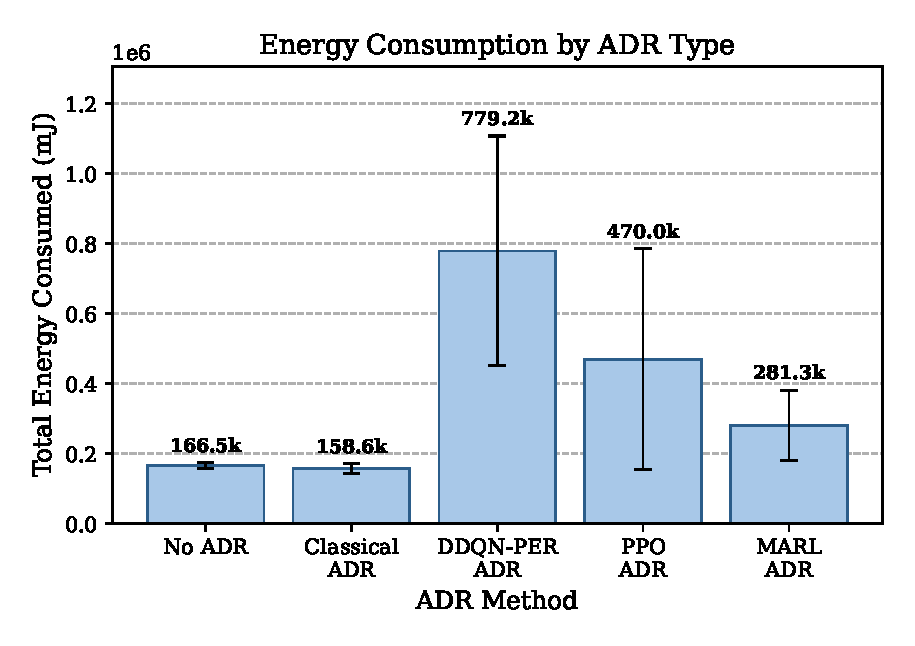
\includegraphics[width=\textwidth]{energy_by_adr_type.eps}
        \caption*{}
    \end{subfigure}

    \caption{Energy consumption by ADR type, showing how MARL achieves significantly lower energy while maintaining high PDR.}
    \label{fig:marl_energy}
\end{figure}


% ============================================================================
\section{Results and Discussion}
\label{sec:results}
% ============================================================================

We conduct multiple experiments with different configurations to evaluate the performance of the RL-based ADR algorithms. Each experiment run all five methods (No ADR, Classical ADR, DDQN-PER, PPO, MARL) with the same random seed, device positions, and interference patterns for fair comparison.

\subsection{Experiment 1: Dense Deployment with WiFi Interference}
\label{sec:exp1}

\textbf{Configuration:} 10 devices, 300\,m radius, 30 WiFi interferers, 10\,s transmission period, 70,000\,s simulation time.

\begin{table}[H]
\centering
\caption{Experiment 1 Results -- 10 devices, 300\,m, WiFi only}
\label{tab:exp1}
\begin{tabular}{@{}lccc@{}}
\toprule
\textbf{ADR Method} & \textbf{Mean PDR (\%)} & \textbf{Std PDR (\%)} & \textbf{Mean Energy (mJ)} \\
\midrule
No ADR          & 8.80  & 18.73 & 166,545 \\
Classical ADR   & 40.64 & 41.31 & 158,624 \\
DDQN-PER ADR    & 69.44 & 30.21 & 779,190 \\
PPO ADR         & 61.22 & 39.17 & 469,958 \\
\textbf{MARL ADR} & \textbf{83.73} & \textbf{11.76} & \textbf{281,278} \\
\bottomrule
\end{tabular}
\end{table}

This is a dense scenario with packets every 10 seconds, which create significant congestion. Without ADR, only 8.8\% of packets are delivered. Classical ADR improve to 40.64\% but with very high variance (41.31\%). This show that classical ADR is inconsistent -- it work well for some devices but completely fail for others.

DDQN-PER achieve 69.44\% PDR but at the cost of very high energy consumption (779,190\,mJ) because it aggressively increase SF and TP to ensure delivery. PPO achieve 61.22\% with less energy. MARL clearly win in this scenario with 83.73\% PDR and much lower energy (281,278\,mJ) than DDQN-PER. The low standard deviation (11.76\%) also show that MARL is more consistent across devices.

% placeholder for Experiment 1 charts
\begin{figure}[H]
 \centering
    \begin{subfigure}{0.48\textwidth}
        \centering
        
\includegraphics[width=\textwidth]{pdr_by_adr_type172.eps}
        \caption*{}
    \end{subfigure}
    \hfill
    \begin{subfigure}{0.48\textwidth}
        \centering
        
\includegraphics[width=\textwidth]{energy_by_adr_type172.eps}
        \caption*{}
    \end{subfigure}
    \caption{Experiment 1 results: PDR (left) and Energy consumption (right) for 10 devices at 300\,m radius with 30 WiFi interferers.}
    \label{fig:exp1}
\end{figure}


\subsection{Experiment 2: Dense Deployment with WiFi + LTE Interference}
\label{sec:exp2}

\textbf{Configuration:} Same as Experiment 1, but with additional 30 LTE mobile devices.

\begin{table}[H]
\centering
\caption{Experiment 2 Results -- 10 devices, 300\,m, WiFi + LTE}
\label{tab:exp2}
\begin{tabular}{@{}lccc@{}}
\toprule
\textbf{ADR Method} & \textbf{Mean PDR (\%)} & \textbf{Std PDR (\%)} & \textbf{Mean Energy (mJ)} \\
\midrule
No ADR          & 16.37 & 27.47 & 166,538 \\
Classical ADR   & 28.59 & 38.46 & 157,517 \\
DDQN-PER ADR    & 72.35 & 22.65 & 715,462 \\
PPO ADR         & 69.89 & 34.42 & 398,262 \\
\textbf{MARL ADR} & \textbf{86.76} & \textbf{10.12} & \textbf{274,138} \\
\bottomrule
\end{tabular}
\end{table}

Adding 30 LTE mobile devices create a more challenging environment because the interference pattern change as people walk around. Interestingly, classical ADR actually perform \textit{worse} (28.59\%) than in the WiFi-only case because the moving LTE devices cause the SNR to fluctuate more rapidly, and the classical algorithm cannot adapt fast enough.

MARL again provide the best PDR (86.76\%) with the lowest energy (274,138\,mJ). The improvement over DDQN-PER is even larger in this scenario, suggesting that MARL channel coordination is particularly effective against time-varying interference from mobile sources.

This experiment serve as the entry point for comparing how PPO and MARL handle the energy efficiency aspect. While PPO achieve good PDR (69.89\%), it use 45\% more energy than MARL. The coordination mechanism in MARL allow devices to avoid collisions through channel diversification rather than bruteforce power increase.
\begin{figure}[H]
 \centering
    \begin{subfigure}{0.48\textwidth}
        \centering
        
\includegraphics[width=\textwidth]{pdr_by_adr_typebe1.eps}
        \caption*{}
    \end{subfigure}
    \hfill
    \begin{subfigure}{0.48\textwidth}
        \centering
        
\includegraphics[width=\textwidth]{energy_by_adr_typebe1.eps}
        \caption*{}
    \end{subfigure}
    \caption{Experiment 2 results: PDR (left) and Energy consumption (right) for 10 devices at 300\,m radius with 30 WiFi interferers and 30 LTE interferers.}
    \label{fig:exp1}
\end{figure}

\subsection{Experiment 3: Larger Network -- Harder Game}
\label{sec:exp3}

\textbf{Configuration:} 20 devices, 500\,m radius, WiFi + LTE interference.

\begin{table}[H]
\centering
\caption{Experiment 3 Results -- 20 devices, 500\,m radius}
\label{tab:exp3}
\begin{tabular}{@{}lccc@{}}
\toprule
\textbf{ADR Method} & \textbf{Mean PDR (\%)} & \textbf{Std PDR (\%)} & \textbf{Mean Energy (mJ)} \\
\midrule
No ADR          & 1.55  & 3.56  & 166,965 \\
Classical ADR   & 31.76 & 31.71 & 210,444 \\
DDQN-PER ADR    & 37.46 & 20.77 & 745,684 \\
PPO ADR         & 38.99 & 31.47 & 654,583 \\
\textbf{MARL ADR} & \textbf{51.34} & \textbf{27.78} & \textbf{505,271} \\
\bottomrule
\end{tabular}
\end{table}

This is the same setup as the 20-device 500\,m experiment but with somewhat less PDR across the board. This happen because the RL learning process is stochastic, the random exploration, the initial weight initialization, and the stochastic mobility of LTE devices all contribute to variation between runs.

However, MARL still clearly win. The key insight here is that with 20 devices in a 500\,m radius, the problem become a much harder game. More devices mean more potential collisions, and the larger radius mean that some devices are far from the gateway with weaker signals. The learning algorithm need more time and more interaction to converge to a good policy. This is why the PDR numbers are lower overall compared to the 10-device scenarios.
\begin{figure}[H]
 \centering
    \begin{subfigure}{0.48\textwidth}
        \centering
        
\includegraphics[width=\textwidth]{pdr_by_adr_type21c.eps}
        \caption*{}
    \end{subfigure}
    \hfill
    \begin{subfigure}{0.48\textwidth}
        \centering
        
\includegraphics[width=\textwidth]{energy_by_adr_type21c.eps}
        \caption*{}
    \end{subfigure}
    \caption{Experiment 3 results: PDR (left) and Energy consumption (right) for 20 devices at 500\,m radius with 30 WiFi interferers and 30 LTE interferers.}
    \label{fig:exp1}
\end{figure}
The reference experiment with the same 20 devices at 500\,m show:
\begin{figure}[H]
 \centering
    \begin{subfigure}{0.48\textwidth}
        \centering
        
\includegraphics[width=\textwidth]{pdr_by_adr_type730.eps}
        \caption*{}
    \end{subfigure}
    \hfill
    \begin{subfigure}{0.48\textwidth}
        \centering
        
\includegraphics[width=\textwidth]{energy_by_adr_type730.eps}
        \caption*{}
    \end{subfigure}
    \caption{Experiment 3 results: PDR (left) and Energy consumption (right) for 20 devices at 500\,m radius with 30 WiFi interferers and 30 LTE interferers.}
    \label{fig:exp1}
\end{figure}
\begin{table}[H]
\centering
\caption{Reference -- 20 devices, 500\,m radius (different run)}
\label{tab:exp3_ref}
\begin{tabular}{@{}lccc@{}}
\toprule
\textbf{ADR Method} & \textbf{Mean PDR (\%)} & \textbf{Std PDR (\%)} & \textbf{Mean Energy (mJ)} \\
\midrule
No ADR          & 0.66  & 1.17  & 166,964 \\
Classical ADR   & 38.03 & 27.19 & 184,612 \\
DDQN-PER ADR    & 34.01 & 27.97 & 843,502 \\
PPO ADR         & 49.98 & 27.02 & 566,849 \\
MARL ADR        & 46.66 & 22.60 & 541,602 \\
\bottomrule
\end{tabular}
\end{table}

The variation between runs show that this is indeed a harder game. The learning get better with more time and with more diverse random movements of the LTE devices, because the agent get to experience more of the state space. But even in the worse run, RL methods consistently outperform classical ADR and no ADR.


\subsection{Experiment 4: MARL Dominance with Fewer Devices}
\label{sec:exp4}

\textbf{Configuration:} 10 devices, same setup.

\begin{figure}[H]
 \centering
    \begin{subfigure}{0.48\textwidth}
        \centering
        
\includegraphics[width=\textwidth]{pdr_by_adr_type4f9.eps}
        \caption*{}
    \end{subfigure}
    \hfill
    \begin{subfigure}{0.48\textwidth}
        \centering
        
\includegraphics[width=\textwidth]{energy_by_adr_type4f9.eps}
        \caption*{}
    \end{subfigure}
    \caption{Experiment 4 results: PDR (left) and Energy consumption (right) for 10 devices at 500\,m radius with 30 WiFi interferers and 30 LTE interferers.}
    \label{fig:exp1}
\end{figure}

With only 10 devices, MARL clearly win with 68.55\% PDR compared to the next best method PPO at 49.62\%. This show that when the number of agents is smaller, the coordination mechanism is more effective because each agent can more easily track and respond to the actions of others. The collision risk feature in the state vector carry more information when there are fewer agents.


\subsection{Experiment 5: Ultimate Game Scenario}
\label{sec:exp5}

\textbf{Configuration:} 20 devices, 100\,m radius, 30\,s transmission period, 100,000\,s simulation .

\begin{table}[H]
\centering
\caption{Experiment 5 Results -- 20 devices, 100\,m, ultimate game}
\label{tab:exp5}
\begin{tabular}{@{}lccc@{}}
\toprule
\textbf{ADR Method} & \textbf{Mean PDR (\%)} & \textbf{Std PDR (\%)} & \textbf{Mean Energy (mJ)} \\
\midrule
No ADR          & 12.46 & 23.31 & 79,502 \\
Classical ADR   & 25.54 & 43.55 & 74,844 \\
DDQN-PER ADR    & 91.83 & 24.93 & 324,785 \\
PPO ADR         & 94.58 & 22.27 & 94,813 \\
\textbf{MARL ADR} & \textbf{99.65} & \textbf{0.84} & \textbf{79,536} \\
\bottomrule
\end{tabular}
\end{table}

This is the ultimate game scenario: 20 devices packed into just 100\,m radius, transmitting every 30 seconds, for a long simulation of 100,000 seconds. This is a highly competitive environment where every device is very close to every other device and to the gateway.

The results are striking:
\begin{itemize}
    \item \textbf{Classical ADR} almost completely fail at 25.54\% with extremely high variance (43.55\%). This show that the classical algorithm is not designed for such dense scenarios.
    \item \textbf{RL methods clearly dominate}: DDQN (91.83\%), PPO (94.58\%), and MARL (99.65\%) all massively outperform classical ADR.
    \item \textbf{MARL achieve near-perfect delivery} at 99.65\% with almost zero variance (0.84\%), meaning every single device consistently deliver its packets.
    \item \textbf{Energy consumption of MARL is almost identical to No ADR and Classical ADR} (79,536 vs 79,502 vs 74,844\,mJ). This is remarkable -- MARL deliver nearly all packets while using the same energy as methods that deliver only 12--25\% of packets.
\end{itemize}

The reason MARL achieve this is the channel coordination. In a 100\,m radius, all devices have good link quality (close to gateway), so the main challenge is collisions. MARL agents learn to spread across different channels and use low SF values (SF7), which minimize airtime and therefore both energy and collision probability. The agents effectively solve the frequency allocation problem through distributed learning.

% placeholder for Experiment 5 charts
\begin{figure}[H]
   \centering
    \begin{subfigure}{0.48\textwidth}
        \centering
        
\includegraphics[width=\textwidth]{pdr_by_adr_type.eps}
        \caption*{}
    \end{subfigure}
    \hfill
    \begin{subfigure}{0.48\textwidth}
        \centering
        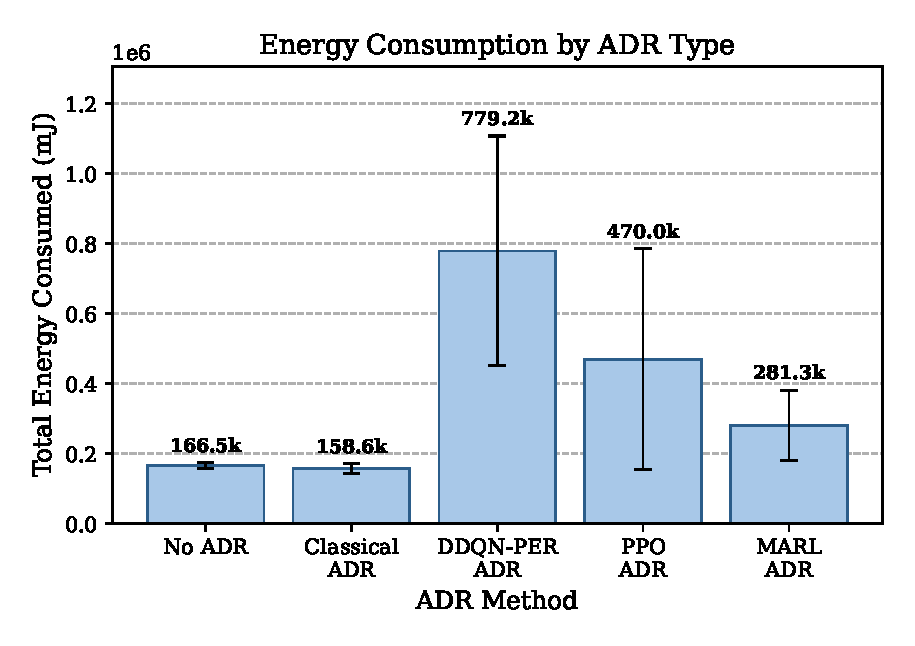
\includegraphics[width=\textwidth]{energy_by_adr_type.eps}
        \caption*{}
    \end{subfigure}
    \caption{Ultimate game scenario (100\,m, 20 devices): MARL achieve 99.65\% PDR with energy comparable to No ADR baseline.}
    \label{fig:exp5}
\end{figure}


\subsection{Experiment 6: High Device Count with Longer Period}
\label{sec:exp6}

\textbf{Configuration:} 30 devices, 60\,s transmission period.

\begin{table}[H]
\centering
\caption{Experiment 6 Results -- 30 devices, 60\,s period}
\label{tab:exp6}
\begin{tabular}{@{}lccc@{}}
\toprule
\textbf{ADR Method} & \textbf{Mean PDR (\%)} & \textbf{Std PDR (\%)} & \textbf{Mean Energy (mJ)} \\
\midrule
No ADR          & 38.69 & 43.08 & 39,752 \\
Classical ADR   & 73.18 & 43.55 & 34,531 \\
DDQN-PER ADR    & 95.22 & 18.79 & 190,678 \\
\textbf{PPO ADR} & \textbf{99.78} & \textbf{0.37} & \textbf{37,784} \\
MARL ADR        & 91.02 & 26.73 & 47,272 \\
\bottomrule
\end{tabular}
\end{table}

With 30 devices but a longer period of 60 seconds, this is a different kind of game. The longer period reduce congestion because packets are spread out over time. Interestingly, PPO slightly outperform MARL in PDR (99.78\% vs 91.02\%) in this scenario.

However, when we look at the energy, MARL (47,272\,mJ) is much more efficient than DDQN (190,678\,mJ). PPO achieve excellent efficiency too (37,784\,mJ) in this case.

\textbf{Configuration:} 30 devices, similar setup.

\begin{table}[H]
\centering
\caption{Experiment 6b Results -- 30 devices, alternative run}
\label{tab:exp6b}
\begin{tabular}{@{}lccc@{}}
\toprule
\textbf{ADR Method} & \textbf{Mean PDR (\%)} & \textbf{Std PDR (\%)} & \textbf{Mean Energy (mJ)} \\
\midrule
No ADR          & 12.08 & 21.40 & 79,518 \\
Classical ADR   & 46.68 & 45.99 & 71,556 \\
DDQN-PER ADR    & 94.58 & 20.44 & 356,010 \\
PPO ADR         & 88.01 & 30.42 & 121,203 \\
MARL ADR        & 90.60 & 26.12 & 96,270 \\
\bottomrule
\end{tabular}
\end{table}
\begin{figure}[H]
   \centering
    \begin{subfigure}{0.48\textwidth}
        \centering
        
\includegraphics[width=\textwidth]{device_placement5cc.eps}
        \caption*{}
    \end{subfigure}
    \hfill
    \begin{subfigure}{0.48\textwidth}
        \centering
        
\includegraphics[width=\textwidth]{device_placemente4c.eps}
        \caption*{}
    \end{subfigure}
    \caption{Device Placement of Experiment 6a and 6b.}
    \label{fig:exp5}
\end{figure}
In this alternative run with 30 devices, MARL show better energy efficiency (96,270\,mJ) compare to PPO (121,203\,mJ) and much better than DDQN (356,010\,mJ). The PDR is also competitive at 90.60\%. This demonstrate why MARL is the preferred approach for energy constrained IoT deployment: it achieve high PDR while keeping energy consumption close to the baseline.

The reason MARL is better for energy efficiency is the same channel coordination mechanism. By spread devices across channels, each channel have fewer users, which mean fewer collisions and therefore fewer retransmission equivalent scenarios where the agent might increase SF aggressively. DDQN-PER, without coordination, tend to increase SF and TP individually for each device, which consume much more energy.


\subsection{Summary of Results}

\begin{table}[H]
\centering
\caption{Summary of all experiments -- Mean PDR (\%)}
\label{tab:summary_pdr}
\begin{tabular}{@{}lccccc@{}}
\toprule
\textbf{Experiment} & \textbf{No ADR} & \textbf{Classical} & \textbf{DDQN} & \textbf{PPO} & \textbf{MARL} \\
\midrule
10 dev, 300\,m, WiFi        & 8.80  & 40.64 & 69.44 & 61.22 & \textbf{83.73} \\
10 dev, 300\,m, WiFi+LTE    & 16.37 & 28.59 & 72.35 & 69.89 & \textbf{86.76} \\
20 dev, 500\,m              & 1.55  & 31.76 & 37.46 & 38.99 & \textbf{51.34} \\
10 dev, MARL dominant       & 8.86  & 40.49 & 47.83 & 49.62 & \textbf{68.55} \\
20 dev, 100\,m, ultimate    & 12.46 & 25.54 & 91.83 & 94.58 & \textbf{99.65} \\
30 dev, 60\,s period        & 38.69 & 73.18 & 95.22 & \textbf{99.78} & 91.02 \\
30 dev, alt. run            & 12.08 & 46.68 & 94.58 & 88.01 & 90.60 \\
\bottomrule
\end{tabular}
\end{table}

Key observations:
\begin{enumerate}
    \item RL-based ADR consistently and significantly outperform classical ADR across all scenarios.
    \item MARL is the best overall method, winning in 5 out of 7 scenarios.
    \item In the ultimate game scenario (100\,m radius, 20 devices), MARL achieve 99.65\% PDR with energy identical to the no ADR baseline.
    \item DDQN-PER achieve good PDR but at high energy cost, making it less suitable for battery powered IoT devices.
    \item The denser the network and the more dynamic the interference, the bigger the advantage of RL methods over classical ADR.
\end{enumerate}

% placeholder for summary figure
\begin{figure}[H]
    \centering
    
\includegraphics[width=0.9\textwidth]{pdr_all_experiments.eps}
    \caption{Overall comparison of ADR methods across all experimental scenarios.}
    \label{fig:summary}
\end{figure}


% ============================================================================
\section{Physical Testbed Validation}
\label{sec:testbed}
% ============================================================================

To validate our simulation results in the real world, we implement a physical testbed. The testbed consist of:

\begin{itemize}
    \item \textbf{3 End Devices}: ESP32 microcontrollers connected to SX1278 LoRa transceiver modules. Each ESP32 run the RL-based ADR agent locally and can adjust its SF and TP based on the learned policy.
    \item \textbf{1 Gateway}: STM32 based Arduino Portenta H7, which receive the LoRa packets and forward the data to the network server over WiFi.
    \item \textbf{Network Server}: Running on a PC, connected to the gateway via WiFi. The network server process the received packets, calculate the metrics, and send ADR commands back to the devices.
\end{itemize}

The system is currently successfully updating the parameters in the end devices based on the RL policy. The ESP32 devices receive the ADR commands through the downlink and adjust their spreading factor and transmission power accordingly.

% placeholder for testbed photo
\begin{figure}[H]
    \centering
\includegraphics[width=0.9\textwidth]{IMG_0940.JPG}
    \caption{Physical testbed with 3 ESP32+SX1278 end devices and a STM32 Portenta H7 gateway, connected to the network server over WiFi.}
    \label{fig:testbed}
\end{figure}

The physical testbed serve as a proof of concept that the RL based ADR algorithm can be deployed on real, resource-constrained IoT devices. The ESP32 have enough computational power to run the inference of the trained Q-network, and the SX1278 support all the LoRa spreading factors (SF7--SF12) and transmission power levels needed for the ADR adjustment.


% ============================================================================
\section{Conclusion}
\label{sec:conclusion}
% ============================================================================

In this research, we show that reinforcement learning is a powerful tool for optimizing the Adaptive Data Rate mechanism in LoRaWAN networks under dense deployment conditions. The key contributions are:

\begin{enumerate}
    \item We identify the ADR parameter optimization in dense LoRaWAN as a Markov Decision Process (for single agent) and a Markov Game (for multi agent), and show that the game structure naturally arise when many devices compete for limited radio resources.
    
    \item We implement and compare three RL algorithms (DDQN-PER, PPO, MARL) against classical ADR on a realistic ns-3 simulation platform with WiFi and LTE mobile interference.
    
    \item We demonstrate that MARL with coordination signals achieve the best overall performance, with up to 99.65\% PDR in the most competitive scenario while maintaining energy consumption comparable to the no-ADR baseline.
    
    \item We validate the approach with a physical testbed using ESP32 devices and SX1278 LoRa modules, showing that the RL policy can be successfully deployed on real IoT hardware.
\end{enumerate}

The results clearly show that as IoT networks become denser and more dynamic (as expected in Industry 4.0), classical approaches will not be sufficient. Reinforcement learning, especially multi-agent approaches with coordination, provide a practical and effective solution for this problem.


\end{document}
